\subsection{Алгоритмы получения и работы с данными батиметрии}

Методы учета шоалинга и рефракции волн, описанные в разделах~\ref{sec:seashoaring} и~\ref{sec:wave_refraction}, требуют для своего выполнения анализа батиметрии в прибрежной зоне.
В разделе~\ref{sec:bathy_source} были рассмотрены принципиально доступные источники батиметрических данных.
Эмпирический опыт реализации инструментов доступа к этим данным позволил выделить два удобных сервиса для их получения: GEBCO и EMODnet.

Доступ к глобальной батиметрической модели GEBCO был реализован через открытый API OpenTopography, единственным ограничением доступа к которому является необходимость предварительной регистрации на портале и использование личного ключа доступа.

Батиметрия прибрежной зоны в западной части России частично покрывается европейской моделью EMODnet, границы которой можно оценить по рисунку~\ref{pic:emodnet} на странице~\pageref{pic:emodnet}.
Модель рельефа дна, распространяется через сервис OGC Web Coverage Service EMODnet Bathymetry, доступ к которой является полностью свободным и не требует выполнения дополнительных условий.

В обоих случаях, для заданных прямоугольных областей (по широте и долготе) по API запрашиваются фрагменты модели и сохраняются в формате \texttt{GeoTIFF}, после чего они считываются в виде регулярной сетки глубин с заданными массивами широт и долгот. 
В процессе чтения значения отсутствующих данных заменяются на пропуски, а координатные массивы формируются так, чтобы каждый элемент матрицы глубин однозначно соответствовал конкретной паре широта-долгота.

Оба источника данных возвращают цифровые модели рельефа описывающие не только морское дно, но и прилегающую сушу, позволяя рассматривать их как единую поверхность.
В единой регулярной сетке соседствуют ячейки с отрицательными значениями глубины (акватории) и положительными отметками высот (континентальная поверхность), благодаря чему легко выделить морские территории по этому признаку.

Тем не менее, в рассматриваемых моделях данные представлены с различным пространственным разрешением.
Глобальная модель GEBCO ориентирована на обеспечение всемирного покрытия и имеет сравнительно крупное разрешение, относительно модель EMODnet Bathymetry, из чего выбор последней является более предпочтительным.
Разница в пространственном разрешении моделей продемонстрирована на рисунке~\ref{pic:NVRSK_GEBCO_EMODnet_bayhtmetry}.

\begin{figure}
    \begin{center}
	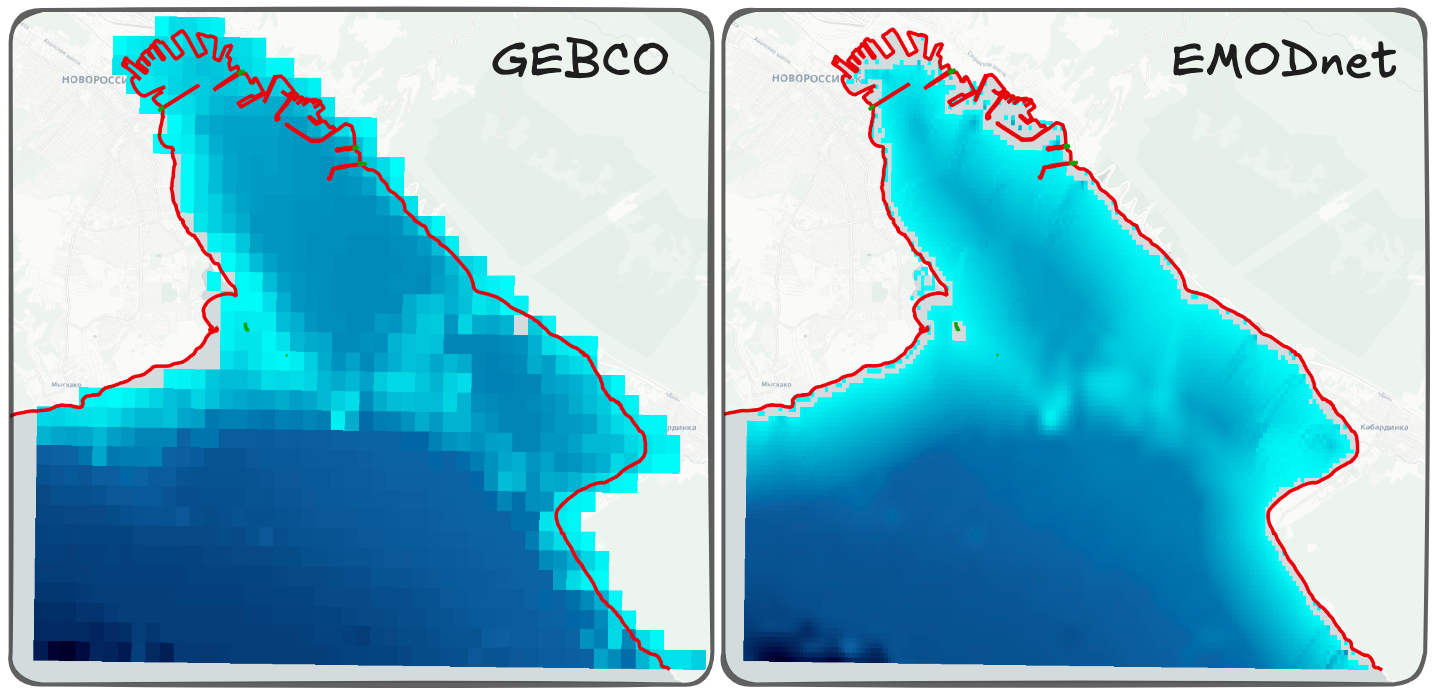
\includegraphics[width=120mm]{fig/part_2/alghoritm/NVRSK_GEBCO_EMODnet_bayhtmetry.png}
	\caption{-- Сравнение пространственного разрешения моделей батиметрии GEBCO и EMODnet}
	\label{pic:NVRSK_GEBCO_EMODnet_bayhtmetry}
    \end{center}
\end{figure}

Для автоматизации выбора источника батиметрических данных в зависимости от географического положения области расчета в программе был реализован фабричный класс, использующая простую логическую схему: если прямоугольная область интереса полностью попадает в заранее заданный контур покрытия EMODnet, то для ее обслуживания выбирается загрузчик EMODnet WCS, в противном случае используется загрузчик глобальной модели GEBCO через сервис OpenTopography.

Для последующего использования батиметрических данных был реализован набор специализированных классов, обеспечивающих полный цикл работы с цифровой моделью рельефа -- от загрузки и интерполяции до построения профилей, необходимых для расчета шоалинга и рефракции.

Для снижения влияния низкого пространственного разрешения моделей в программе реализован функционал линейной интерполяции глубины в произвольной точке относительно соседних для нее ячеек растра.
Интерполяция реализована как для одиночных точек, так и для массивов точек, что особенно важно при вычислении профиля дна, выполняемого при анализе шоалинга.
В результате, модели расчета, использующие батиметрию, получают доступ к непрерывной поверхности глубин, а не только к значениям в узлах исходной сетки.
Реализованные алгоритмы интерполяции приближают результаты GEBCO модели к EMODnet, что можно визуально оценить на рисунке~\ref{pic:GEBCO_EMODnet_difference}.

\begin{figure}
    \begin{center}
	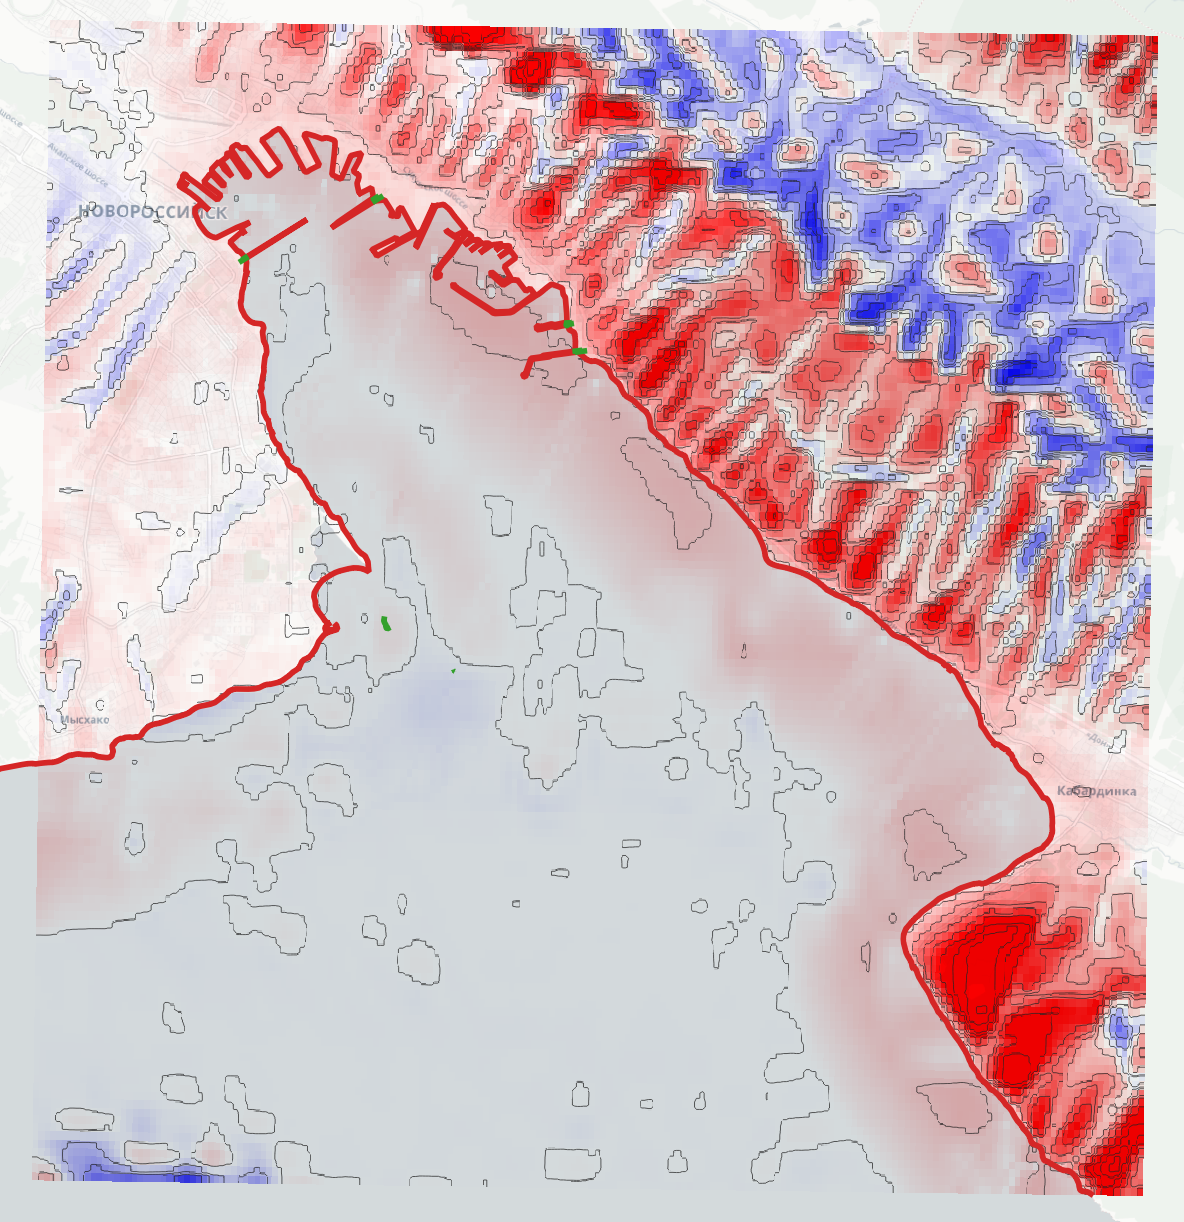
\includegraphics[width=100mm]{fig/part_2/alghoritm/GEBCO_EMODnet_difference.png}
	\caption{-- Разность между проинтерполиированными моделями GEBCO и EMODnet}
	\label{pic:GEBCO_EMODnet_difference}
    \end{center}
\end{figure}

В совокупности разработанные классы обеспечивают единообразный и воспроизводимый подход к работе с батиметрическими данными независимо от их источника.
